\frame
{
	\frametitle{Distributed Online Learning for Large-Scale Patterns Prediction}
	%\framesubtitle{Maritime Surveillance}
	\framesubtitle{Proposed System Model}
	\begin{center}
		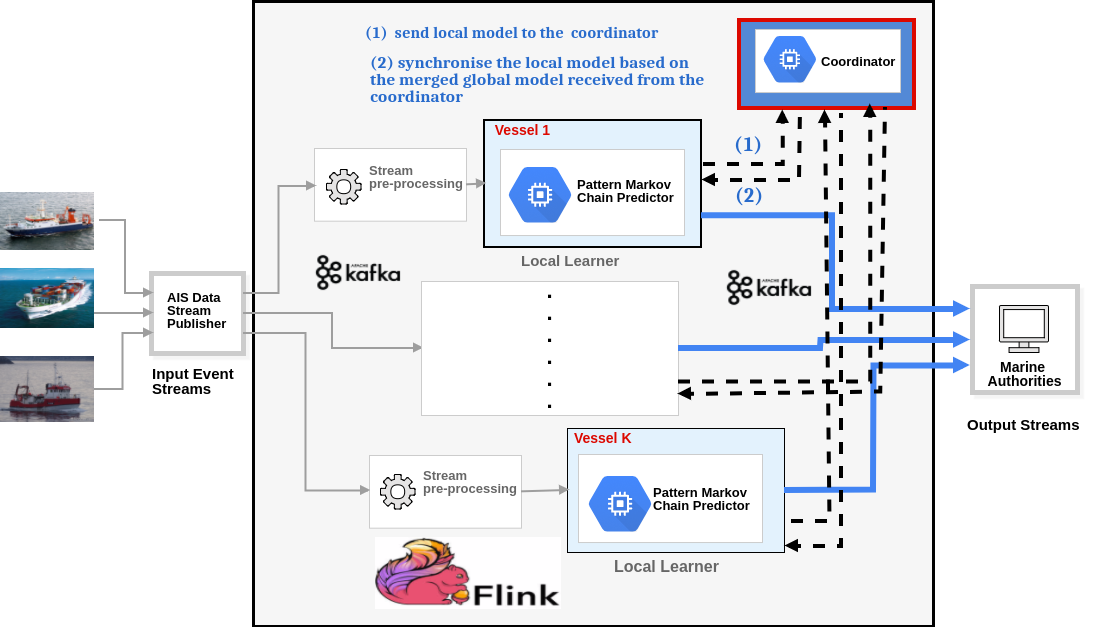
\includegraphics[width=1.05\textwidth,left]{figures/architecturedist_v2.png}\\
.
	\end{center}
}


\frame
{
	\frametitle{ Communication-Efficient Distributed Online Prediction by Dynamic Model Synchronization  }
	\framesubtitle{\citep{kamp2014communication}}
	\begin{itemize}[]
		\item<1-> A protocol for distributed online prediction over multiple input data streams in a communication efficient manner.
		\item<1-> It allows to combine local models into a global model
	using a $synchronization$ $ operation$.
		\item<1-> The distributed learners exchange their local model with a central coordinator node periodically after observing a fixed number of data points (i.e., mini-batches) \citep{dekel2012optimal}.
		
		\item<1-> A dynamic synchronization scheme based on monitoring the local models variance from a global reference model ($\|f_i - r\|^2 \leq \bigtriangleup$).
		
		
%		dynamic synchronization scheme within which the learners communicate only if their local models diverge from a global reference point
	\end{itemize}
}

\frame
{
	\frametitle{Distributed Online Learning for Large-Scale Patterns Prediction}
		\framesubtitle{Proposed Synchronization Operation}
	\begin{itemize}[]

	\item<1-> The
 $synchronization$ $ operater$ of the local maximum likelihood estimator as the following:
 \begin{equation*}
 \label{eq:pi_estim}
 \hat{p}_{i,j}=\frac{\sum_{k \in K} n_{k,i,j}}{\sum_{k \in K} \sum_{l \in L} n_{k,i,l}}
 \end{equation*}

	
\end{itemize}
}